%%%%%%%%%%%%%%%%%%%%%%%%%%%%%%%%%%%%%%%%%%%%%%%%%%%%%%%%%%%%%%%%%%%%%%%%%%%%%%
%%Skeleton LaTeX file: double column format.
%%%%%%%%%%%%%%%%%%%%%%%%%%%%%%%%%%%%%%%%%%%%%%%%%%%%%%%%%%%%
%%REMEMBER THAT THERES IS AN EIGHT PAGE SIZE RESTRICTION
%%%%%%%%%%%%%%%%%%%%%%%%%%%%%%%%%%%%%%%%%%%%%%%%%%%%%%%%%%%%

%%% Sample file for ME Project Papers for Evaluation by Supervisor and Reader

\documentclass{article}

\usepackage{multicol}
\usepackage{graphicx}

\pagestyle{empty}
\setlength{\topmargin}{ 0.25in}
\setlength{\columnsep}{2.0pc}
\setlength{\headheight}{0.0in}
\setlength{\headsep}{0.0in}
\setlength{\oddsidemargin}{-.19in}
\setlength{\parindent}{1pc}
\textheight 8.75in
\textwidth 6.8in

\title{\large \bf Predicting Query Execution Time }
\author{Name}

\date{}

\begin{document}

	\maketitle
    \begin{center}
        Mid-term ME Project Report
    \end{center}
        \vskip 12pt
	\thispagestyle{empty}
	\bibliographystyle{unsrt}
		\begin{abstract}
		The ability to estimate the query execution time is central for a number of tasks in database system
		such as query scheduling, progress monitoring and costing during query optimization. Recent work 
		has explored the use of statistical techniques in place of the manually constructed cost models used 
		in query optimization. Such techniques, which require as training data along with the 
		actual execution time, promises superior accuracies for they being able to account the for factors 
		such as hardware characteristics and bias in cardinality estimates. However, such techniques fail 
		to generalize i.e., produce poor estimates for queries that are not seen during the training.
		
		In this work, we propose and evaluate predictive modeling techniques that learn query 
		execution behavior at a fine grained operator level. For each operator, we consider different sets 
		of features and build different models for them. Since there are only finitely many operators in 
		database, this approach is practical and will be able to estimate any query as its a composition of
		many operators. We evaluate our approaches using TPC-H and TPC-DS workloads on PostgreSQL.

	\end{abstract}		
	\hfill 
	\begin{multicols}{2}
	\section{INTRODUCTION}
	Database systems can greatly benefit from accurate execution time predictions including: 
	Explain the application briefly here.
	\begin{itemize}
	\item Query Optimizer: 
	\item Query Scheduling:
	\item Progress monitoring:
	\end{itemize}
	If possible plot a non-linear SVR for the data. will the optimizer's cost 
	itself is enough 1D regression using linear, polynomial and RBF kernels
	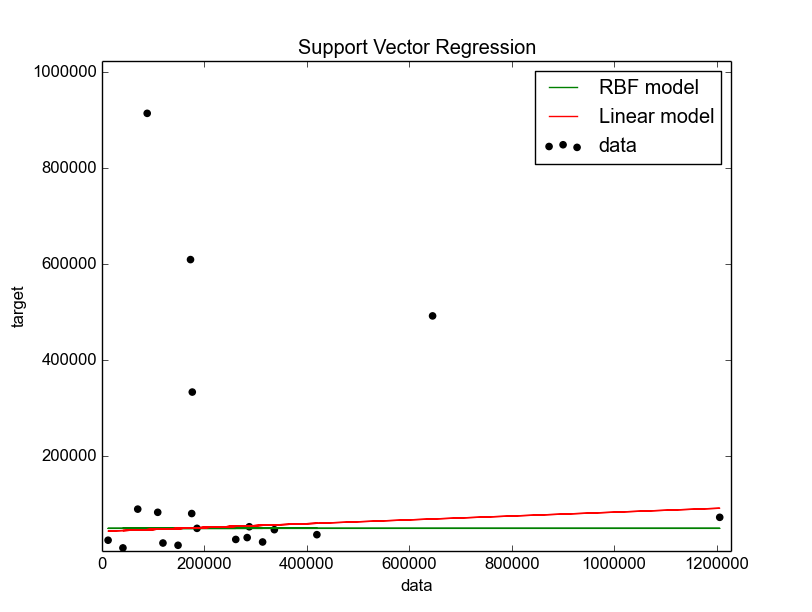
\includegraphics[scale=.33]{optcost.png}  
	\section{Overview}
	Elaborate what is the plan level approach. give  a intro model
	 based techniques. i.e.,  OFF LINE TRAINING, emphasize one time.
	1. How to obtain training data (explain analyze)
	2. getting execution times at plan nodes
	3. Individual model training 
	4. Explain while testing and predict using Model more in next section
%%%%%%%%%%%%%  This can be followed by several other sections
	\section{Model selection and Training}
	What model is considered good ? choice of model and kernel
	If possible prove linear systems are not sufficient.
	Training data ,specification. Does more training data helps?
	 training time etc.. 
	Essentially all operators need to be covered. generation QGEN tool. 
	\section{Preliminary Experiments}
	Give a background about Static and dynamic workload.  
	do experiments at 2 stages
	1. Act vs Act
	2. Est vs Est(Bias towards estimated cardinalities)
	For each type of above scenario, do testing for tpc-h queries 
	(tpc-ds in future)
	At different scales to see the model's ability to predict.
	For midterm you should be having result for 1 as well as 10 GB.
	For each above dataset, 
	Results should convey L1 (MRE) as well as queries that are within 
	[0-0.5] [0.5-1] [1-1.5] 
	\section{Conclusions and Future Work}
	Talk about generalization. 
	operator specific features
	capturing query interaction i.e., pipeline source of over-estimation
	Optimizers provides sufficient information to detect a pipeline,
	 can we use it to bind the operators and predict execution time 
	 for a set of operators instead of a single operator.
	
    \bibliographystyle{abbrv}
    \bibliography{}
	
	\end{multicols}
\end{document}
